\documentclass[12pt]{beamer}

\usepackage[english]{babel}
\usepackage[utf8]{inputenc}
\usepackage{tikz}

\usetheme{Copenhagen}
\setbeamertemplate{navigation symbols}{}

\usetikzlibrary{snakes}
\tikzstyle{event}=[circle,fill=black!100,inner sep=0pt,minimum size=3pt]
\tikzstyle{message}=[->,snake=coil,segment aspect=0,segment length=20pt]
\tikzstyle{tick}=[draw=black!80,dashed]
\tikzstyle{process}=[circle,draw=black!100]
\tikzstyle{resource}=[rectangle,draw=black!100]
\tikzstyle{scheduler}=[draw=black!100,dotted]

\title[Times, Clocks and the ordering of Events]{Times, Clocks, and the Ordering of Events in a Distributed System}
\author[Jacopo Notarstefano]{
    Jacopo Notarstefano\\
    \texttt{jacopo.notarstefano [at] gmail.com}
}
\date{13 February 2013}

\begin{document}
    \begin{frame}[plain]
        \titlepage
    \end{frame}

    \begin{frame}{Main objectives and outline}
        In this paper Lamport:
        \begin{enumerate}
            \item gives a distributed algorithm for extending the partial
            ordering defined by the ``happened before'' relation to a consistent
            total ordering of all the events,
            \item uses this algorithm to solve a mutual exclusion problem.
        \end{enumerate}
    \end{frame}

    \begin{frame}{Distributed system}
        \begin{definition}[Distributed system]
            A \emph{distributed system} consists of a collection of distinct processes
            which are ``spatially separated'', and which communicate with one another
            by exchanging messages.

            A system is distributed if the message transmission delay is not
            negligible compared to the time between events in a single process.
        \end{definition}
    \end{frame}

    \begin{frame}{Examples of distributed systems}
        \begin{itemize}
            \item A worldwide network of interconnected computers
            \item A cluster of workstation in a data center
            \item Processes on a single computer
        \end{itemize}
    \end{frame}

    \begin{frame}{Review of ordering relations}
        \begin{definition}[Partial order]
            A \emph{partial order} \(\le_{P}\) on a set \(X\) is a reflexive, antisymmetric,
            transitive relation.
        \end{definition}
        \begin{definition}[Total order]
            A \emph{total order} \(\le\) on a set \(X\) is a partial order such that, if
            \(a,b\in X\), then either \(a\le b\) or \(b\le a\).
        \end{definition}
        \begin{definition}[Linear extension]
            We say that a total order \(\le\) on \(X\) \emph{extends} a partial order
            \(\le_{P}\) if \(\forall a,b\in X\) we have \(a\le_{P}b\Rightarrow a\le b\).
        \end{definition}
    \end{frame}

    \begin{frame}{The ``\(\rightarrow\)'' relation}
        \begin{definition}[The ``\(\rightarrow\)'' relation]
            The ``\(\rightarrow\)'' relation on the set of events of a system
            is the smallest relation satisfying the following three conditions:
            \begin{enumerate}
                \item If \(a\) and \(b\) are events in the same process, and
                \(a\) comes before \(b\), then \(a \rightarrow b\).
                \item If \(a\) is the sending of a message by one process,
                and \(b\) is the receipt of the same message by another
                process, then \(a \rightarrow b\).
                \item If \(a \rightarrow b\), and \(b \rightarrow c\), then
                \(a \rightarrow c\).
            \end{enumerate}
        \end{definition} 
    \end{frame}

    \begin{frame}{The space-time diagram}
        \begin{figure}
            \makebox[\textwidth][c]{
              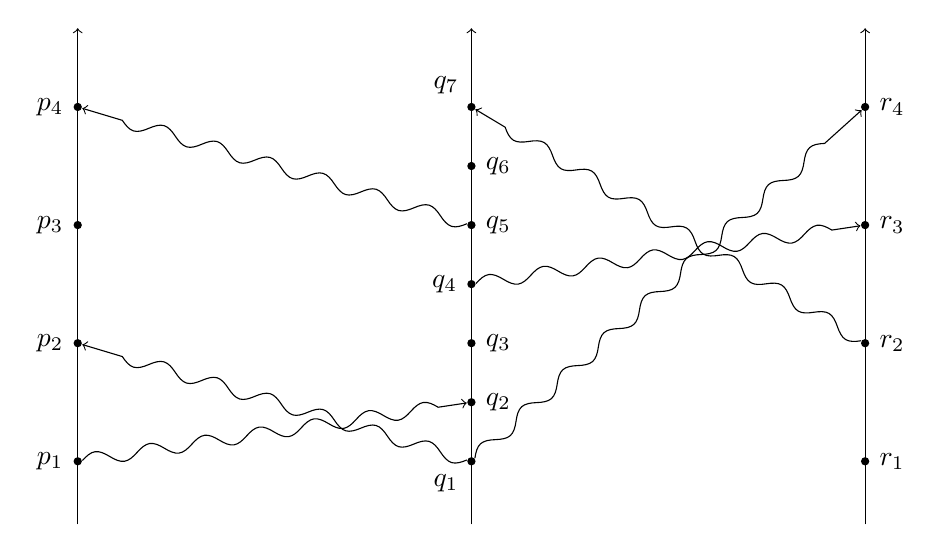
\begin{tikzpicture}
                  \draw [->] (0,0.7) -- (0,7);
                  \draw [->] (5,0.7) -- (5,7);
                  \draw [->] (10,0.7) -- (10,7);

                  \node (p1) at (0,1.5) [event,label=180:{$p_1$}] {};
                  \node (p2) at (0,3) [event,label=180:{$p_2$}] {};
                  \node (p3) at (0,4.5) [event,label=180:{$p_3$}] {};
                  \node (p4) at (0,6) [event,label=180:{$p_4$}] {};

                  \node (q1) at (5,1.5) [event,label=225:{$q_1$}] {};
                  \node (q2) at (5,2.25) [event,label=0:{$q_2$}] {};
                  \node (q3) at (5,3) [event,label=0:{$q_3$}] {};
                  \node (q4) at (5,3.75) [event,label=180:{$q_4$}] {};
                  \node (q5) at (5,4.5) [event,label=0:{$q_5$}] {};
                  \node (q6) at (5,5.25) [event,label=0:{$q_6$}] {};
                  \node (q7) at (5,6) [event,label=135:{$q_7$}] {};

                  \node (r1) at (10,1.5) [event,label=0:{$r_1$}] {};
                  \node (r2) at (10,3) [event,label=0:{$r_2$}] {};
                  \node (r3) at (10,4.5) [event,label=0:{$r_3$}] {};
                  \node (r4) at (10,6) [event,label=0:{$r_4$}] {};

                  \draw [message] (p1) -- (q2);
                  \draw [message] (q1) -- (p2);
                  \draw [message] (q5) -- (p4);

                  \draw [message] (q1) -- (r4);
                  \draw [message] (q4) -- (r3);
                  \draw [message] (r2) -- (q7);
              \end{tikzpicture}
            }
        \end{figure}
    \end{frame}

    \begin{frame}{Clocks}
        \begin{definition}[Clock]
            For each process \(P_i\) we define a \emph{clock} \(C_i\) to be a
            function that assigns a number \(C_i\langle a\rangle\) to
            each event \(a\) in the process.
        \end{definition}

        \begin{definition}[System of clocks]
            A \emph{system of clocks} is a function \(C\) that assigns to the
            event \(b\) in process \(P_j\) the time \(C\langle b\rangle =
            C_j\langle b\rangle\).
        \end{definition}
    \end{frame}

    \begin{frame}{The clock condition}
        \begin{definition}[The clock condition]
            We say that a system of clocks satisfies the \emph{clock condition}
            if, for any events \(a\) and \(b\), we have: if \(a\rightarrow b\)
            then \(C\langle a\rangle < C\langle b\rangle\).
        \end{definition}

        \begin{lemma}
            The clock condition is satisfied if the following conditions hold:
            \begin{enumerate}
                \item If \(a\) and \(b\) are events in process \(P_i\) and \(a\)
                comes before \(b\), then \(C_i\langle a\rangle < C_i\langle b\rangle\).
                \item If \(a\) is the sending of a message by process \(P_i\) and \(b\)
                is the receipt of that message by process \(P_j\), then
                \(C_i\langle a\rangle < C_j\langle b\rangle\).
            \end{enumerate}
        \end{lemma}
    \end{frame}

    \begin{frame}{Implementation of the clock condition}
        \begin{lemma}
            To guarantee that a system of clocks satisfies the clock condition we
            need to obey the following implementation rules:
            \begin{enumerate}
                \item Each process \(P_i\) increments \(C_i\) between any two
                successive events.
                \item If event \(a\) is the sending of a message \(m\) by process
                \(P_i\), then the message \(m\) contains a timestamp
                \(T_m = C_i\langle a\rangle\).
                \item Upon receiving a message \(m\), process \(P_j\) sets \(C_j\)
                greater than or equal to its present value and greater than \(T_m\).
            \end{enumerate}
        \end{lemma}
    \end{frame}

    \begin{frame}{The space-time diagram, revisited}
        \begin{figure}
            \makebox[\textwidth][c]{
              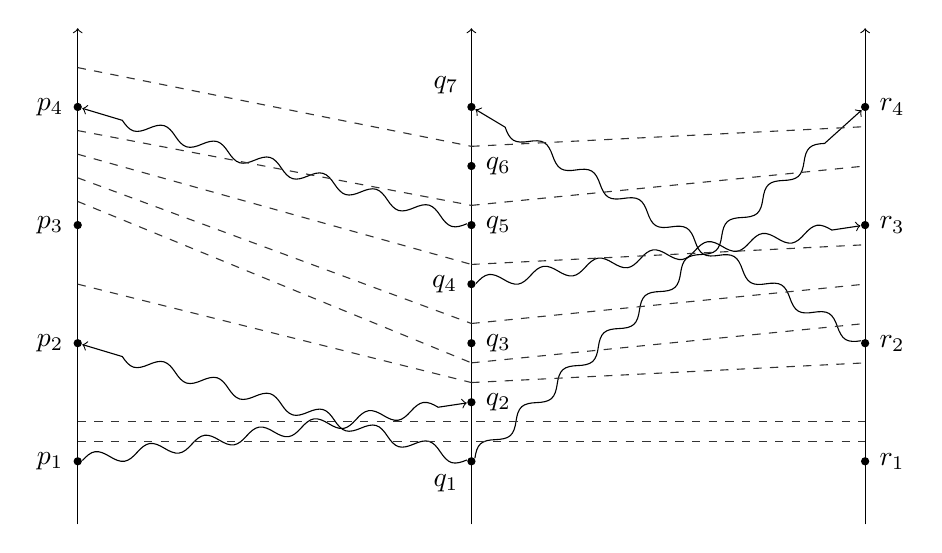
\begin{tikzpicture}
                  \draw [->] (0,0.7) -- (0,7);
                  \draw [->] (5,0.7) -- (5,7);
                  \draw [->] (10,0.7) -- (10,7);

                  \node (p1) at (0,1.5) [event,label=180:{$p_1$}] {};
                  \node (p2) at (0,3) [event,label=180:{$p_2$}] {};
                  \node (p3) at (0,4.5) [event,label=180:{$p_3$}] {};
                  \node (p4) at (0,6) [event,label=180:{$p_4$}] {};

                  \node (q1) at (5,1.5) [event,label=225:{$q_1$}] {};
                  \node (q2) at (5,2.25) [event,label=0:{$q_2$}] {};
                  \node (q3) at (5,3) [event,label=0:{$q_3$}] {};
                  \node (q4) at (5,3.75) [event,label=180:{$q_4$}] {};
                  \node (q5) at (5,4.5) [event,label=0:{$q_5$}] {};
                  \node (q6) at (5,5.25) [event,label=0:{$q_6$}] {};
                  \node (q7) at (5,6) [event,label=135:{$q_7$}] {};

                  \node (r1) at (10,1.5) [event,label=0:{$r_1$}] {};
                  \node (r2) at (10,3) [event,label=0:{$r_2$}] {};
                  \node (r3) at (10,4.5) [event,label=0:{$r_3$}] {};
                  \node (r4) at (10,6) [event,label=0:{$r_4$}] {};

                  \draw [message] (p1) -- (q2);
                  \draw [message] (q1) -- (p2);
                  \draw [message] (q5) -- (p4);

                  \draw [message] (q1) -- (r4);
                  \draw [message] (q4) -- (r3);
                  \draw [message] (r2) -- (q7);

                  \draw [tick] (0,1.75) -- (10,1.75);
                  \draw [tick] (0,2) -- (10,2);
                  \draw [tick] (0,3.75) -- (5,2.5);
                  \draw [tick] (5,2.5) -- (10,2.75);
                  \draw [tick] (0,4.8) -- (5,2.75);
                  \draw [tick] (5,2.75) -- (10,3.25);
                  \draw [tick] (0,5.1) -- (5,3.25);
                  \draw [tick] (5,3.25) -- (10,3.75);
                  \draw [tick] (0,5.4) -- (5,4);
                  \draw [tick] (5,4) -- (10,4.25);
                  \draw [tick] (0,5.7) -- (5,4.75);
                  \draw [tick] (5,4.75) -- (10,5.25);
                  \draw [tick] (0,6.5) -- (5,5.5);
                  \draw [tick] (5,5.5) -- (10,5.75);
              \end{tikzpicture}
            }
        \end{figure}
    \end{frame}

    \begin{frame}{The space-time diagram, rearranged}
        \begin{figure}
            \makebox[\textwidth][c]{
              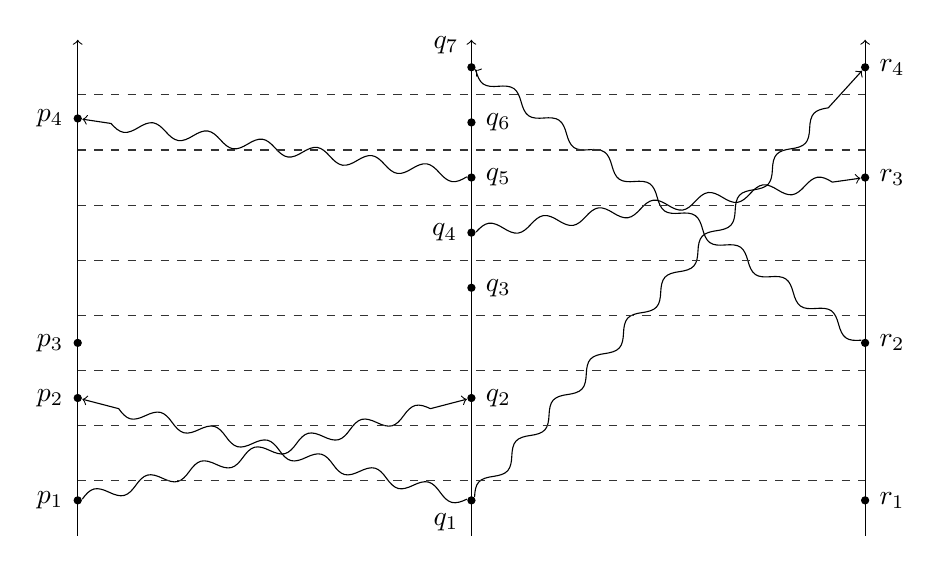
\begin{tikzpicture}
                  \draw [->] (0,0.7) -- (0,7);
                  \draw [->] (5,0.7) -- (5,7);
                  \draw [->] (10,0.7) -- (10,7);

                  \node (p1) at (0,1.15) [event,label=180:{$p_1$}] {};
                  \node (p2) at (0,2.45) [event,label=180:{$p_2$}] {};
                  \node (p3) at (0,3.15) [event,label=180:{$p_3$}] {};
                  \node (p4) at (0,6) [event,label=180:{$p_4$}] {};

                  \node (q1) at (5,1.15) [event,label=225:{$q_1$}] {};
                  \node (q2) at (5,2.45) [event,label=0:{$q_2$}] {};
                  \node (q3) at (5,3.85) [event,label=0:{$q_3$}] {};
                  \node (q4) at (5,4.55) [event,label=180:{$q_4$}] {};
                  \node (q5) at (5,5.25) [event,label=0:{$q_5$}] {};
                  \node (q6) at (5,5.95) [event,label=0:{$q_6$}] {};
                  \node (q7) at (5,6.65) [event,label=135:{$q_7$}] {};

                  \node (r1) at (10,1.15) [event,label=0:{$r_1$}] {};
                  \node (r2) at (10,3.15) [event,label=0:{$r_2$}] {};
                  \node (r3) at (10,5.25) [event,label=0:{$r_3$}] {};
                  \node (r4) at (10,6.65) [event,label=0:{$r_4$}] {};

                  \draw [message] (p1) -- (q2);
                  \draw [message] (q1) -- (p2);
                  \draw [message] (q5) -- (p4);

                  \draw [message] (q1) -- (r4);
                  \draw [message] (q4) -- (r3);
                  \draw [message] (r2) -- (q7);

                  \draw [tick] (0,1.4) -- (10,1.4);
                  \draw [tick] (0,2.1) -- (10,2.1);
                  \draw [tick] (0,2.8) -- (10,2.8);
                  \draw [tick] (0,3.5) -- (10,3.5);
                  \draw [tick] (0,4.2) -- (10,4.2);
                  \draw [tick] (0,4.9) -- (10,4.9);
                  \draw [tick] (0,5.6) -- (10,5.6);
                  \draw [tick] (0,6.3) -- (10,6.3);
              \end{tikzpicture}
            }
        \end{figure}
    \end{frame}

    \begin{frame}{The ``\(\Rightarrow\)'' relation}
        \begin{definition}[The ``\(\Rightarrow\)'' relation]
            Let \(\le\) be a total ordering on the processes. If \(a\) is an
            event in process \(P_i\) and \(b\) is an event in process \(P_j\), then
            \(a\Rightarrow b\) if and only if either
            \begin{enumerate}
                \item \(C_i\langle a\rangle < C_j\langle b\rangle\) or
                \item \(C_i\langle a\rangle = C_j\langle b\rangle\) and
                \(P_i\le P_j\).
            \end{enumerate}
        \end{definition}
    \end{frame}

    \begin{frame}{A mutual exclusion problem}
        A fixed collection of processes share a single resource, which can be used
        by one process at a time. We want to find an algorithm that satisfies
        the following conditions:
        \begin{enumerate}
            \item A process which has been granted the resource must release it before
            it can be granted to another process.
            \item Different requests for the resource must be granted in the order in
            which they are made.
            \item If every process which is granted the resource eventually releases
            it, then every request is eventually granted.
        \end{enumerate}
    \end{frame}

    \begin{frame}{A wrong solution, 1/3}
        We can't elect a  central scheduling process which grants requests in
        the order they are received. Suppose that \(p_1\) sends a message to
        \(p_0\), the scheduler, to request the resource \(R\).
        \begin{figure}
            \makebox[\textwidth][c]{
                \begin{tikzpicture}
                    \node (r) at (4,3.464) [resource] {$R$};
                    \node (p0) at (2,3.464) [process] {$p_0$};
                    \node (p1) at (0,0) [process] {$p_1$};
                    \node (p2) at (4,0) [process] {$p_2$};

                    \draw [scheduler] (p0) -- (r);
                    \draw [message] (p1) -- (0.5,0.866);
                \end{tikzpicture}
            }
        \end{figure}
    \end{frame}

    \begin{frame}{A wrong solution, 2/3}
        Then \(p_1\) sends a message to \(p_2\). Suppose that this message is
        received while the other is still traveling due to network congestion.
        \begin{figure}
            \makebox[\textwidth][c]{
                \begin{tikzpicture}
                    \node (r) at (4,3.464) [resource] {$R$};
                    \node (p0) at (2,3.464) [process] {$p_0$};
                    \node (p1) at (0,0) [process] {$p_1$};
                    \node (p2) at (4,0) [process] {$p_2$};

                    \draw [scheduler] (p0) -- (r);
                    \draw [message] (p1) -- (1,1.732);
                    \draw [message] (p1) -- (p2);
                \end{tikzpicture}
            }
        \end{figure}
    \end{frame}

    \begin{frame}{A wrong solution, 3/3}
        Finally, \(p_2\) sends a message to \(p_0\) requesting the resource.
        \(p_0\) then grants the resource to \(p_2\), which requested the
        resource after \(p_1\).
        \begin{figure}
            \makebox[\textwidth][c]{
                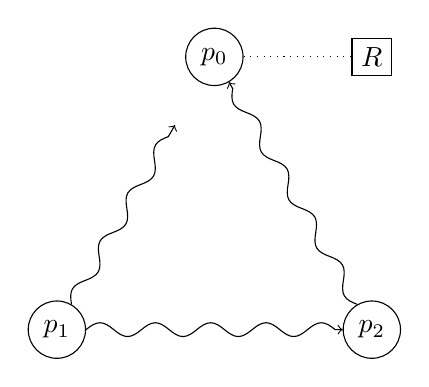
\begin{tikzpicture}
                    \node (r) at (4,3.464) [resource] {$R$};
                    \node (p0) at (2,3.464) [process] {$p_0$};
                    \node (p1) at (0,0) [process] {$p_1$};
                    \node (p2) at (4,0) [process] {$p_2$};

                    \draw [scheduler] (p0) -- (r);
                    \draw [message] (p1) -- (1.5,2.598);
                    \draw [message] (p1) -- (p2);
                    \draw [message] (p2) -- (p0);
                \end{tikzpicture}
            }
        \end{figure}
    \end{frame}

    \begin{frame}{Some assumptions}
        To simplify the problem, we make some assumptions.
        \begin{enumerate}
            \item For any two processes \(P_i\) and \(P_j\), the messages sent from
            \(P_i\) to \(P_j\) are received in the same order as they are sent.
            \item Every message is eventually received.
            \item A process can send messages directly to every other process.
        \end{enumerate}
    \end{frame}

    \begin{frame}{The request queue}
        Let \(P_0\) be the process to which the shared resource is initially allocated.
        Let \(T_0\) be less than the initial value of any logical clock in the system.
        Each process mantains a private \emph{request queue}, which initially contains
        one message: ``\(T_0\): \(P_0\) requests resource''.
    \end{frame}

    \begin{frame}{Resource request and acknowledgment}
        \begin{enumerate}
            \item Process \(P_i\) sends the message ``\(T_m\): \(P_i\) requests
            resource'' to every other process where \(T_m\) is the process clock's value
            at the time of the request. \(P_i\) also puts the request message on its
            request queue.
            \item When process \(P_j\) receives \(P_i\)'s request message, it puts it
            in its queue and sends an acknowledgment message to \(P_i\).
        \end{enumerate}
    \end{frame}

    \begin{frame}{Resource release and acknowledgement}
        \begin{enumerate}
            \setcounter{enumi}{2}
            \item Process \(P_i\) removes request message ``\(T_m\): \(P_i\) requests
            resource'' from its queue and sends the release message ``\(P_i\) releases
            resource'' to every other process.
            \item Process \(P_j\) removes the ``\(T_m\): \(P_i\) requests resource''
            from its queue.
        \end{enumerate}
    \end{frame}

    \begin{frame}{Resource allocation}
        \begin{enumerate}
            \setcounter{enumi}{4}
            \item Process \(P_i\) is granted the resource when:
            \begin{itemize}
                \item There is a ``\(T_m\): \(P_i\) requests resource'' in \(P_i\)'s request
                queue which is before any other request according to \(\Rightarrow\).
                \item \(P_i\) has received messages from every other process timestamped
                later than \(T_m\).
            \end{itemize}
        \end{enumerate}
    \end{frame}

    \begin{frame}{Proof of correctness (sketch)}
        \begin{theorem}
            The algorithm described by rules \(1\) to \(5\) is a correct solution to the
            mutual exclusion problem.
        \end{theorem}
        \begin{proof}[Proof (sketch)]
            The ordering is guaranteed by the fact that relation ``\(\Rightarrow\)''
            extends relation ``\(\rightarrow\)''.
        \end{proof}
    \end{frame}
\end{document}
